\chapter{Terminologi}
\label{kap:terminologi} % Opprinnelig kapittelnr: A

\section{Indekser og summasjoner}


Gitt en liste bestående av $n$ tall
\[ x_1, x_2, \ldots , x_n \]
slik at $x_i$ er det $i$'te tallet på listen. Her kaller vi $i$ en indeks 
eller fotskrift. Summen av de $n$ tallene skriver vi
\[ x_1 + x_2 + \cdots + x_n \]
Det er vanlig å la symbolet $\Sigma$ bety ``summen av". Vi har derfor følgende 
alternative skrivemåte
\[ \sum_{i=1}^{n} x_i   \]
som leses ``summen av alle $x_i$'er fra $i=1$ til $i=n$".

I denne forbindelse blir indeksen $i$ også kalt summasjonsindeksen.
Det er likegyldig hvilken bokstav som brukes, mest vanlig er likevel $i$,
$j$, $k$, $l$, $m$ og $n$.Vi må imidlertid passe på at vi ikke velger en
summasjonsindeks som også er brukt i en annen betydning.

Symbolbruken varieres etter behov, eksempelvis
\begin{eqnarray*}
\sum_{i=3}^{n} x_i  &  \mbox{betyr} & 
    \mbox{``summen av alle $x_i$'er fra $i=3$ til $i=n$''},\\
\sum_{i=1}^{n-2} x_i&  \mbox{betyr} & 
    \mbox{``summen av alle $x_i$'er fra $i=3$ til $i=n-2$''},\\
\sum_{j=3}^{5} x_j &  \mbox{betyr}  & 
    \mbox{``summen av alle $x_j$'ene for  $j=3, 4$ og 5''},\\
\sum_{n=k}^{m} x_n &  \mbox{betyr}  & 
    \mbox{``summen av alle $x_n$ fra $n=k$ til $n=m$''}.
\end{eqnarray*}
I noen situasjoner vil de tall som summeres ikke nødvendigvis komme etter
hverandre, vi kan da skrive
\[ \sum_{i\in A} x_i   \]
som leses ``summen av de $x_i$'er med indeks som er med i mengden $A$"
(om mendeterminologi se nedenfor). Eksempelvis dersom $A=\{1,4,5\}$ blir
$\sum_{i\in A} x_i =  x_1 + x_4 + x_5$.

Av og til går det fram av sammenhengen hvilke indekser det skal summeres over,
og vi tillater oss da å skrive
\[ \sum_{i} x_i   \]
Symbolbruken kan også varieres på andre måter etter behov, eksempelvis
\begin{center}
\[ \sum_{i=1}^{n} 2x_i = 2x_1 + 2x_2 + \cdots + 2x_n \]
\[ \sum_{i=1}^{n} (x_i+2) = (x_1+2) + (x_2 + 2) + \cdots + (x_n+2) \]
\[ \sum_{i=1}^{n} x_i^2 = x_1^2 + x_2^2 + \cdots + x_n^2 \]
\[ \sum_{i=1}^{n} f(x_i) = f(x_1) + f(x_2) + \cdots + f(x_n) \]
\[ \sum_{i=1}^{n} i x_i = 1\cdot x_1 + 2 \cdot x_2 + \cdots + n \cdot x_n \]
\[ \sum_{i=1}^{n} x_i f(x_i) = x_1 \cdot f(x_1) + x_2 \cdot f(x_2) + 
                   \cdots + x_n \cdot f(x_n) \]
\[ \sum_{i=1}^{n} (x_i+y_i) = (x_1+y_1) + (x_2 + y_2) + \cdots + (x_n+y_n) \]
\end{center}
Følgende regneregler er verd å merke seg
\[ (a) \mbox{\ \ } \sum_{i} k x_i = k \sum_{i} x_i \mbox{\ \ (k konstant)} \]
\[ (b) \mbox{\ \ } \sum_{i} (x_i + y_i) = \sum_{i} x_i + \sum_{i} y_i \]
som gjelder uansett hvilke indekser det summeres over, bare det er de samme 
på begge sider av likhetstegnet. Det også verd å merke seg at
\[ (c) \mbox{\ \ } \sum_{i} a = a + a + \cdots + a = n \cdot a \]
der $n$ er antall indekser det summeres over.

Disse tre regnereglene kan brukes til å forenkle mer kompliserte summeringer.

I noen situasjoner kan utgangspunktet være en uendelig tallfølge 
$x_1, x_2, x_3, \ldots$. For den uendelige summen
\[ x_1 + x_2 + x_3 + \cdots   \]
brukes vanligvis den forkortede skrivemåten
\[ \sum_{i=1}^{\infty} x_i   \]
Lesere med kunnskaper i matematisk analyse vil vite at slike summer
ikke nødvendigvis gir mening som noe endelig tall.

I enkelte sammenhenger er det aktuelt å summere tallene i et
rektangulært skjema
\begin{center}
\begin{tabular}{cccc}
              $x_{11}$& $x_{12}$& $\cdots$& $x_{1n}$ \\
              $x_{21}$& $x_{22}$& $\cdots$& $x_{2n}$ \\
              $\vdots$& $\vdots$&         & $\vdots$ \\
              $x_{m1}$& $x_{m2}$& $\cdots$& $x_{mn}$
\end{tabular}
\end{center}
slik at $x_{ij}$ betegner tallet i $i$'te linje og $j$'te søyle.
Summen av alle tallene skrives

\[               \sum_{i,j}x_{ij}     \]
der vi summerer over alle indekspar ($i,j$).  Alternative skrivemåter
er 

\[ \sum_{i=1}^m \sum_{j=1}^n x_{ij} = \sum_{j=1}^n \sum_{i=1}^m x_{ij} \]
I uttrykket til venstre skjer summeringen ved først å 
summere over $j$ for hver $i$, og deretter summere over $i$, dvs. vi
summerer hver linje og summerer deretter linjesummene.  I uttrykket
til høyre skjer summeringen i omvendt rekkefølge, først
summeres hver søyle og deretter summeres søylesummene.  Begge
framgangsmåter må gi samme resultat, og hvilken som brukes vil
avhenge av omstendighetene.

Symbolbruken kan også her varieres etter behov, og regneregler
kan etableres.  Vi vil ikke gå i detalj, men nøye oss med et
interessant resultat (la $x_{ij} = a_i\cdot b_i$)

\[ (d) \mbox{\ \ \ } \sum_{i=1}^m \sum_{j=1}^na_i\cdot b_j = (\sum_{i=1}^ma_i)\cdot
     (\sum_{j=1}^nb_j) \]
Summasjonsindeksen behøver ikke alltid være en fotskrift,
i teksten forekommer uttrykk av form

\[ \sum_x f(x) \mbox{\ \ \ } \sum_{x,y}f(x,y) \]
eventuelt med nærmere angivelse av hvilke $x$ (eventuelt $x$ og $y$)
det skal summeres over.


\section{Mengder og funksjoner}
                     
Med en {\em mengde} forstås en samling av objekter, heretter kalt
{\em elementer}.\\

Vi vil benytte store bokstaver, som oftest i begynnelsen av alfabetet, 
til å symbolisere mengder.  For elementer i mengden brukes den
symbolikk som ansees som mest velegnet for det aktuelle formål.
Eksempler på mengder er:
\begin{center}
\begin{tabular}{ll}
$A$ = de ensifrede tall              & = \{0,1,2,$\ldots$ , 9\} \\
$B$ = de to-sifrede tall             & = \{00,01,02,$\ldots$ , 98,99\} \\
$C$ = de norske bokstaver            & = \{a,b,c,$\ldots$ , ø,å\} \\
$D$ = tegnene på en skrivemaskin & = \{a,A,b,B,$\ldots$ ,?,!\} \\
$E$ = elevene i en klasse            & = \{NN,JL,$\ldots$ ,BB\} \\
$N$ = de naturlige tall              & = \{0,1,2,3,$\ldots$ \} \\
$Z$ = de hele tall                   & = \{$\ldots$ ,-3,-2,-1,0,1,2,3,
                                               $\ldots$ \}
\end{tabular} 
\end{center}
Klammen \{\} leses som ``mengden av elementene", og innenfor klammene er
en beskrivelse eller eventuelt en oppramsing av disse elementene.
Rekkefølgen av elementene i en slik oppramsing er likegyldig,
eksempelvis er \{1,2,3,\} og \{2,1,3\} samme mengde.  I de situasjoner der
elementene i mengden har en naturlig rekkefølge er denne brukt for
å lette oversikten.  Skriver vi

\[     M = \{e_1, e_2, \ldots, e_n\}         \]
betyr dette mengden bestående av elementene $e_1,e_2, \ldots e_n$,
rekkefølgen er likegyldig.  I enkelte situasjoner er det 
hensiktsmessig å skrive

\[         M = \{e; \mbox{``$e$ oppfyller betingelsen ...''} \} \]% 
som leses``mengden av alle elementer $e$ slik at $e$ oppfyller 
betingelsen $\ldots$".

En mengde som består av et endelig antall elementer kalles en
{\em endelig mengde}.  Vi ser at mengdene $A, B, C, D$ og $E$ ovenfor
er endelige mengder, mens $N$ og $Z$ er {\em uendelige mengder}.  Andre
eksempler på uendelige mengder er
\begin{center}
\begin{tabular}{rcl}
      O &=& alle odde tall \\
      Q &=& de rasjonale tall \\
      R &=& de reelle tall
\end{tabular}
\end{center}
En {\em tellbar} mengde (også kalt diskret mengde) er en mengde der
elementene lar seg nummerere med naturlige tall, element nr.1, element 
nr.2 osv.  Alle endelige mengder er tellbare, noen uendelige mengder
er tellbare, andre ikke.  $N$ og $O$ ovenfor er opplagt tellbare mengder,
og det kan vises at også $Z$ og $Q$ er tellbare.  $R$ er derimot
ikke tellbar, vi sier at de reelle tall er en {\em overtellbar} mengde
(også kalt kontinuerlig mengde).

Symbolkombinasjonen

\[           e\in M         \]
leser vi ``$e$ er et element i mengden $M$".  Eksempelvis er 
$4\in A$, $13\in B$, $u\in C$, $?\in D$, $JL\in E$, $696\in N$, $-4\in Z$,
$3/8\in Q$, $\sqrt{2}\in R$.

Er to mengder $A$ og $B$ slik at ethvert element i $A$ også er med
i $B$ sier vi at $A$ er en {\em delmengde} (eller undermengde) av $B$
og skriver $A\subset B$.  Eksempelvis er $A\subset N, O\subset N,
N\subset Q$ og $Q\subset R$.

Det er ofte bruk for å utføre regneoperasjoner på mengder.
De mest vanlige regneoperasjonene er {\em union, snitt} og 
{\em komplement}.  Det finnes en rekke regneregler som angår disse
regneoperasjonene.  Definisjonene og de regnereglene som er 
nødvendige for vårt formål er gitt i teksten.

\begin{quote}
En regel som til ethvert element i en mengde $M_1$ tilordner et og bare et 
element i en annen mengde $M_2$ kaller vi en {\em funksjon} fra 
$M_1$ til $M_2$.
\end{quote}
La $f$ være en funksjon fra $M_1$ til $M_2$, symbolisert slik
         
\[       f : M_1\rightarrow M_2   \]
Her kalles $M_1$ {\em definisjonsmengden} (definisjonsområdet)
og $M_2$ {\em målmengden}.  Når $x$ er et vilkårlig element
i $M_1$ vil $f(x)\in M_2$ være verdien av funksjonen $f$ for
elementet $x$.  I denne forbindelse brukes også skrivemåten

\[          f: x\rightarrow f(x)  \]
som sier at $f$ er den regel som til elementet $x$ tilordner 
elementet $f(x)$.\\[0.5cm]

Eksempler på funksjoner er

\indent $M_1 = B$, $M_2 = B$ og $f$ = summen av sifrene  \\
\indent $M_1 = C$, $M_2 = N$ og $f$ = bokstavens nr. i alfabetet \\
\indent $M_1 = E$, $M_2 = A$ og $f$ = elevens karakter på en prøve.\\

I mange anvendelser vil $M_1$ og $M_2$ være delmengder av de reelle
tall.  Eksempler på funksjoner er da 
\begin{center}
\begin{tabular}{crl}
        &  $f$: & $x\rightarrow x+1$ \\
        &  $f$: & $x\rightarrow x^2$ \\
        &  $f$: & $x\rightarrow x^2 - 3x+2$ \\
        &  $f$: & $x\rightarrow logx $
\end{tabular}
\end{center}
Noen mengder kan hensiktsmessig beskrives ved en funksjon.  Her er 

\[      \{x; f(x) = y \} \]
mengden av alle elementer $x$ som tilordnes verdien $y$ ved 
funksjonen $f$.  Eksempelvis kan mengden av alle løsninger av
annengradsligningen \\ $x^2 - 3x + 2 = 0$ skrives

\[        \{x; x^2 - 3x + 2 = 0\}  \]
som for øvrig er lik \{1,2\}.  Likeens betrakt

\[     \{x; x^2 + 1 = 0\} \]
Siden ligningen $x^2 + 1 = 0$ ikke har noen reell løsning, er denne
mengden uten elementer, vi sier at det er {\em den tomme mengde}
symbolisert med $\emptyset$.



\section{Det greske alfabet}

\begin{center}
\begin{tabular}{|l|cc|l|cc|lcc|} \hline
Skrift & Stor & Liten    &Skrift  & Stor & Liten &Skrift & Stor&Liten\\ \hline
alfa   & A    & $\alpha$  & iota   & I  & $\iota$    & rho & P  & $\rho$   \\
beta   & B    &$\beta$  & kappa  & K  &$\kappa$ & sigma & $\Sigma$ &$\sigma$ \\
gamma  &$\Gamma$&$\gamma$& lambda &$\Lambda$&$\lambda$& tau & T &$\tau$ \\
delta  &$\Delta$&$\delta$& my     & M &$\mu$& ypsilon &$\Upsilon$&$\upsilon$\\
epsilon& E    &$\epsilon$& ny     & N   &$\nu$     & phi &$\Phi$&$\phi$   \\
zeta   & Z    &$\zeta$   & ksi    &$\Xi$&$\xi$     & khi & X  &$\chi$   \\
eta    & H    &$\eta$    & omikron& O   & o        & psi &$\Psi$&$\psi$  \\
theta  &$\Theta$&$\theta$& pi     &$\Pi$&$\pi$   & omega &$\Omega$ &$\omega$ \\
\hline
\end{tabular}
\end{center}

\section{Ordliste: Engelsk - Norsk}
\small
\begin{center}
\begin{tabular}{ll}
Autocorrelation & Autokorrelasjon  \\
Average         & Gjennomsnitt  \\
Biased          & Forventningsskjev \\
Binomial        & Binomisk \\
Chi-square      & Kjikvadrat \\
Cluster         & Klynge \\
Confidence interval & Konfidensintervall \\
Contingency table &   Kontigenstabell \\
Correlation    &  Korrelasjon \\
Covariance      & Kovarians \\
Critical region & Forkastningsområde \\
Critical value  & Kritisk verdi \\
Cumulative distribution & Kumulativ fordeling \\
\end{tabular}
\end{center}
\begin{center}
\begin{tabular}{ll}
Degrees of freedom & Frihetsgrader \\
Density function & Tetthetsfunksjon \\
Design           & Forsøksplan \\
Disjoint         & Disjunkt  \\
Distribution     & Fordeling \\
Error of first kind & Forkastingsfeil \\
Error of second kind & Godtakingsfeil \\
Estimate         & Estimat, estimere \\
Estimator        & Estimator \\
Event            & Begivenhet, hendelse \\
Expectation      & Forventning \\
Frequency        & Hyppighet \\
Forecast         & Prognose, prediksjon \\
Histogram        & Histogram \\
Hypergeometric   & Hypergeometrisk \\
Independence     & Uavhengighet \\
Interaction      & Samspill \\
Intersection     & Snitt \\
Least squares method & Minste kvadraters metode \\
Mean (arithmetic) & Gjennomsnitt \\
Mean             & Forventning \\
Mean square deviation & Empirisk varians, middelkvadratavvik \\
Median           & Median \\
Moving average   & Glidende gjennonsnitt \\
Normal           & Normal \\
Operating characteristic & Karakteristikk \\
Outlier          & Vill observasjon \\
Paired comparison & Parvis sammenligning \\
Parameter        & Parameter \\
Population       & Populasjon \\
Posterior probability & Aposteriori sannsynlighet \\
Power function   & Styrkefunksjon \\
Predictor        & Prediktor \\
Prior probability & Apriori sannsynlighet \\
Probability      & Sannsynlighet \\
Probability measure & Sannsynlighetsmål \\
Quantile         & Fraktil \\
Random           & Stokastisk, tilfeldig \\
Random variable  & Stokastisk variabel \\
Randomisation    & Randomisering \\
Range            & Variasjonsbredde \\
Rank             & Rang, rangordne \\
Ratio estimate   & Rateestimat \\
Regression       & Regresjon \\
Relative frequency & Relativ hyppighet \\
Replacement      & Tilbakelegging \\
Residual         & Residual \\
Robust           & Robust \\
\end{tabular}
\end{center}
\begin{center}
\begin{tabular}{ll}
Sample           & Utvalg, velge ut \\
Sample space     & Utfallsrom \\
Sampling         & Utvelging \\
Sampling plan    & Utvalgsplan \\
Seasonal variation & Sesongvariasjon \\
Serial correlation & Autokorrelasjon \\
Sign test          & Tegn test \\
Significance level & Signifikansnivå \\
Significance probability & P-verdi, signifikanssannsynlighet \\
Significant        & Signifikant \\
Simple event       & Enkel begivenhet \\
Simulation         & Simulering \\
Standard deviation & Standardavvik \\
Standard error     & Standardavvik, standardfeil \\
Stationary         & Stasjonær \\
Statistic          & Observator \\
Statistics         & Statistikk  \\
Stochastic         & Stokastisk, tilfeldig \\
Stratification     & Stratifisering \\
Stratum            & Stratum \\
Sure event         & Sikker begivenhet \\
Survey             & Undersøkelse \\
Test statistic     & Testobservator \\
Tied observations  & Sammenfallende observasjoner \\
Time series        & Tidsrekke \\
Trend              & Trend \\
Trial              & Forsøk \\
Unbiased           & Forventningsrett \\
Variance           & Varians \\
Variance analysis  & Variansanalyse \\
Variate            & Stokastisk variabel \\
\end{tabular}
\end{center}  
\normalsize
Av mer omfattende ordlister nevnes: 
\small
\begin{itemize}
\item[]
Marriott: A Dictionary of Statistical terms.  5.Ed.\\
  Longman Scientific \& Technical, Burnt Hill Harlow Essex, 1990. 
\item[]
Nordisk Statistisk Nomenklatur.  Studentlitteratur, Lund, 1975. \\
\end{itemize}
\normalsize
Den første gir utfyllende forklaringer på engelske termer, den 
andre gir sammenhørende termer på engelsk, norsk og de andre
nordiske språk.

\chapter{Formler}
\addtolength{\baselineskip}{+0.1\baselineskip}
{\bf Aksiomer :}\\ \\
\begin{tabular}{ll}                             
A1.&  $ 0 \leq P(u) \leq 1 \mbox{\ \  for alle utfall \ } u $\\[0.1cm]
A2.&  $   P(u_1)+P(u_2)+P(u_3)+ \cdots =1 $ \\[0.1cm] 
A3.&  $   P(A)=\sum_{u \in A}P(u) $ \\[0.1cm]
A4.&  $   P(u\mid B)=P(u)/P(B)\mbox{\ \ for \ } u\in B \mbox{\ \ (=0 ellers)}$
\end{tabular}\\ \\
{\bf Egenskaper :}\\ \\
\begin{tabular}{ll}
E1.&  $ 0 \leq P(A) \leq 1 \mbox{\ \ for alle begivenheter  } A $ \\[0.1cm] 
E2.&  $    P(\Omega)=1 $ \\[0.1cm] 
E3.&  $ P(A \cup B) = P(A) + P(B)  \mbox{\ \  når}\ \ A \cap B = \emptyset $ \\[0.1cm] 
E4.&  $   P(\bar{A}) = 1-P(A) $ \\[0.1cm]
E5.&  $  P(\emptyset) = 0 $ \\[0.1cm] 
E6.&  $  P(A \cup B) = P(A) + P(B) - P(A \cap B) $ \\[0.1cm] 
E7.&  $P(A_1 \cup A_2 \cup \cdots \cup A_n) =
       P(A_1) + P(A_2) +\cdots + P(A_n) $  når\\[0.1cm] 
   &  $A_1, A_2 \cdots A_n$ er disjunkte begivenheter\\[0.1cm]
E8.&  $ P(A \mid B)=P(A \cap B)/P(B) $\\[0.1cm]
E9.&  $ P(A\cap B)=P(B)\cdot P(A\mid B) $ \\[0.1cm]
E10.& $ P(B \mid A)=P(B) \cdot P(A \mid B)/P(A) $ (Bayes lov) \\[0.1cm]
E11.& $ P(A)=P(B_1)\cdot P(A\mid B_1)+P(B_2)\cdot P(A\mid B_2)+ \cdots +P(B_r)\cdot P(A\mid B_r) $ \\[0.1cm]
   & når $\Omega = B_1 \cup B_2 \cup \cdots \cup B_r)$ er en disjunkt union \\[0.1cm]
E12.& $  P(A\cap B) = P(A) \cdot P(B)$ når $A$ og $B$ er uavhengige
\end{tabular} \\ \\

\noindent {\bf De Morgans lover :} \\ \\
\begin{tabular}{ll}
M1.&  $ \overline{A_1 \cup A_2 \cup \cdots \cup A_n}=
   \bar{A}_1 \cap \bar{A}_2 \cap \cdots \cap \bar{A}_n$ \\[0.1cm]
M2.&  $ \overline{A_1 \cap A_2 \cap \cdots \cap A_n}=
   \bar{A}_1 \cup \bar{A}_2 \cup \cdots \cup \bar{A}_n$ 
\end{tabular} \\ \\
{\bf Kombinatorikk :}\\ \\
\begin{tabular}{ll}
K1.&  ${(N)}_s=N(N-1)(N-2)\cdots (N-s+1)$ \\[0.1cm]
K2.&  $ {N\choose s} =\frac{{(N)}_s}{s!}=\frac{N!}{s!(N-s)!}$\\[0.1cm]
K3.&  $ N!=1\cdot 2\cdot 3\cdots N $
\end{tabular} \\ \\
{\bf Forventning :} \\ \\
\begin{tabular}{ll}
F1.&  $ EX=\sum_{u}X(u)P(u) $ \\[0.1cm]
F2.&  $ EX=\sum_{x}xP(X=x)= \sum_{x}xp(x) $\\[0.1cm]
F3.&  $ E(k)=k  $ \\[0.1cm]
F4.&  $ E(k+X)=k+EX $ \\[0.1cm] 
F5.&  $ E(kX)=k EX $ \\[0.1cm]
F6.&  $ E\phi (X)=\sum_{x}\phi (x)p(x)  $\\[0.1cm]
F7.&  $ E(X+Y)=EX+EY   $\\[0.1cm]
F8.&  $ E(X_1+X_2+\cdots +X_n)=EX_1+EX_2+\cdots +EX_n $\\[0.1cm]
F9.&  $ E(k_0+k_1X_1+k_2X_2+ \cdots +k_nX_n)$           \\[0.1cm]
   &          \hspace{1cm}$= k_0+k_1EX_1+k_2EX_2+ \cdots +k_nEX_n $\\[0.1cm]
F10.& $ E\phi(X,Y)=\sum_{(x,y)}\phi (x,y)p(x,y) $\\[0.1cm]
F11.& $  E(X\cdot Y)=EX\cdot EY
 \mbox{\ \ såframt $X$ og $Y$ er uavhengige.} $\\[0.1cm]
F12.& $ EE(Y\mid X)=EY  $\\[0.1cm]
F13.& $ ES_n=n\cdot EX $\\[0.1cm]
F14.& $ ES_N = EN \cdot EX  $
\end{tabular} \\ \\
\newpage
\noindent {\bf Varians :} \\ \\
\begin{tabular}{ll}
V1.&  $ varX = E(X - \mu)^2 \mbox{\ \ der \ } \mu =EX$\\[0.1cm]
V2.&  $ varX = \sum_{x}{(x-\mu)}^2p(x) $\\[0.1cm]
V3.&  $ varX = E(X^2) - (EX)^2 $\\[0.1cm]
V4.&  $ varX = \sum_{x}x^2p(x)-{(EX)}^2 $\\[0.1cm]
V5.&  $ var(k)=0   \mbox{\ \  (k konstant)} $ \\[0.1cm]
V6.&  $ var(k+X)=var X $\\[0.1cm]
V7.&  $ var(kX)=k^2 varX $\\[0.1cm]
V8.&  $ var(X+Y)=varX+varY+2cov(X,Y) $ \\[0.1cm]
V9.&  $ var(X+Y)=varX+varY
              \mbox{ når $X$ og $Y$ er ukorrelerte} $ \\[0.1cm]
V10.& $ var(\sum_{i=1}^n X_i)= \sum_{i=1}^n var(X_i)
             + \sum_{i \ne j}cov(X_i,X_j)   $\\[0.1cm]
V11.& $ var(\sum_{i=1}^n X_i)= \sum_{i=1}^n var(X_i)$ når $X_i$'ene
                              er ukorrelerte \\[0.1cm]
V12.& $ varS_n = n var X.  $\\[0.1cm]
V13.& $ var S_N = EN\cdot var X + var N\cdot (EX)^2. $ 
\end{tabular}\\ \\

\noindent {\bf Kovarians :} \\ \\
\begin{tabular}{ll}
C1.&  $  cov(X,Y)=E((X-EX)\cdot (Y-EY))  $\\[0.1cm]
C2.&  $ cov(X,Y)=E(X\cdot Y)-EX\cdot EY $\\[0.1cm]
C3.&  $ cov(X,Y)=\sum_{(x,y)}xy \cdot p(x,y)-EX\cdot EY $\\[0.1cm]
C4.&  $ p(x,y)=p_1(x)\cdot p_2(y) \mbox{ medfører } cov(X,Y)=0 $\\[0.1cm]
C5.&  $ \rho (X,Y)=\frac{cov(X,Y)}{\sqrt{varX} \cdot \sqrt{varY}} $
\end{tabular} \\ \\
\newpage

\noindent {\bf Normaltilnærming :} ($\mu=EX$, ${\sigma}^2=varX$)\\ \\
\begin{tabular}{ll}
G1.& $G(-z)=1-G(z)$ \\[0.1cm]
G2.& $P(X\leq x)\approx G(\frac{x-\mu}{\sigma })$\\[0.1cm]
G3.& $P(X>x)=1-P(X\leq x)\approx 1-G(\frac{x-\mu}{\sigma })$\\[0.1cm]
G4.& $P(a<X\leq b)\approx G(\frac{b-\mu}{\sigma })-G(\frac{a-\mu}{\sigma })$\\[0.1cm]
G5.& $P(X\leq x)\approx G(\frac{x+\frac{1}{2}-\mu}{\sigma })$ (heltallsvariabel)\\[0.1cm]
G6.& $ P(\mid X-\mu \mid < k\cdot \sigma)\approx A(k)$\\[0.1cm]
G7.& $ P(\mid X-\mu \mid < d)\approx A(d/\sigma)$
\end{tabular} \\ \\
{\bf Tsjebysjeffs ulikhet :}\\ \\
\begin{tabular}{ll}
T1.& $ P(\mid X-\mu \mid < k\cdot \sigma) \geq 1-1/k^2$
\end{tabular}\\ \\
{\bf Sannsynlighetsfordelinger :} \\ \\
\begin{tabular}{ll}
1.& Binomisk fordeling $(n,p)$ :  $  P(X=x)=\bino{n}{x}p^x{(1-p)}^{n-x} $\\[0.1cm]
  & $ EX=np, \mbox{\ \ \ } varX=np(1-p) $\\ \\
2.& Hypergeometrisk fordeling $(N,M,n)$ :
     $ P(Y=y)= \frac{\bino{M}{y} \cdot \bino{N-M}{n-y}}{\bino{N}{n}} $ \\[0.1cm] 
  & $ EY=n\cdot \frac{M}{N}, \mbox{\ \ \ } varY=\frac{N-n}{N-1}\cdot n\cdot
                                            \frac{M}{N}(1-\frac{M}{N}) $\\ \\ 
3.& Poissonfordeling $(\lambda)$ :  $ P(X=x)=\frac{{\lambda}^x}{x!}e^{-\lambda} $\\[0.1cm]
  & $ EX=\lambda,\mbox{\ \ \ } varX=\lambda$\\ \\
4.& Geometrisk fordeling $(p)$ :  $ P(N=n)={(1-p)}^{n-1} p $\\[0.1cm]
  & $ EN=1/p, \mbox{\ \ \ } varN=(1-p)/p^2 $\\ \\
\end{tabular} \\ \\
\newpage
\noindent {\bf Empiriske mål :}\\ \\
\begin{tabular}{ll}
1.& Gjennomsnitt: $\bar{X} = \frac{1}{n} \sum_{i=1}^{n}X_{i} $\\[0.1cm]
2.& Empirisk varians: $S_X^2 = \frac{1}{n}\sum_{i=1}^{n}(X_{i}-\bar{X})^{2}$\\[0.1cm]
3.& Empirisk standardavvik: $S_X=\sqrt{S_X^2}$\\[0.1cm]
4.& Empirisk kovarians: $S_{XY} =\frac{1}{n} \sum_{i=1}^{n}(X_{i}-\bar{X})\cdot(Y_{i}-\bar{Y}) $\\[0.1cm]
5.& Empirisk korrelasjonskoeffisient: $R_{XY}=\frac{S_{XY}}{S_{X} \cdot S_{Y}}$
\end{tabular}\\ \\
\noindent {\bf Målemodellen :}\\ \\
 $X_1,X_2,\ldots ,X_n$ uavhengige $EX_i=\mu$, $varX_i={\sigma}^2$.
 \[E\bar{X}=\mu, \mbox{\ \ \ }var\bar{X}=\frac{{\sigma}^2}{n}\]
{\bf Lotterimodellen :}\\ \\
 $Y_1,Y_2,\ldots ,Y_n$ tilfeldig utvalg fra $v_1,v_2,\ldots ,v_N$ .
\[ E\bar{Y}=\bar{v}, \mbox{\ \ \ } 
                  var\bar{Y}=\frac{N-n}{N-1}\cdot \frac{{\sigma}^2}{n}\]
der \ \ ${\sigma}^2=\frac{1}{N}\sum_{i=1}^N {(v_i-\bar{v})}^2.$

\addtolength{\baselineskip}{-0.1\baselineskip}

\chapter{Tabeller}
\label{app:fordelngstabeller}

\begin{table}[H]
\centering
  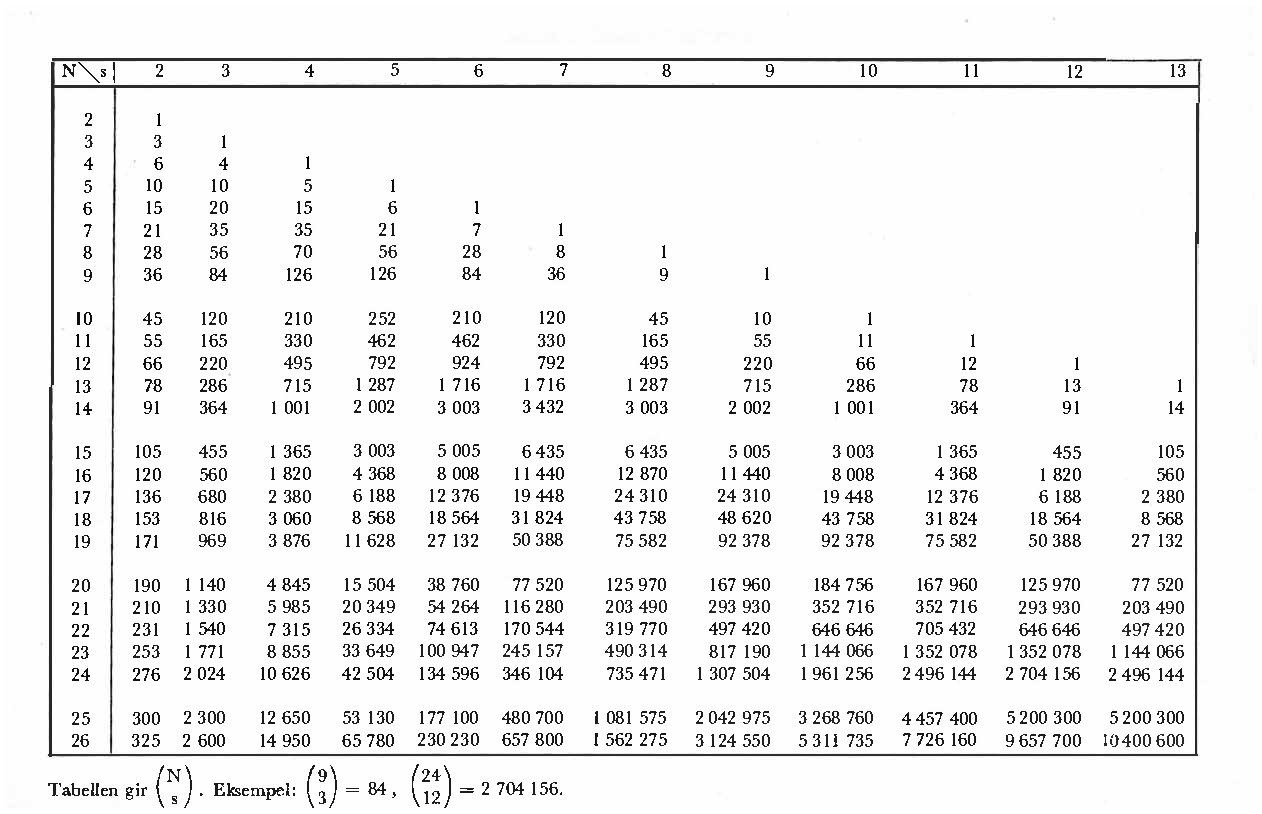
\includegraphics[scale=0.8]{figurer/Tabell_1_Binomiske_koeffisienter.pdf}
 \caption{Binomiske koeffisienter}
 \label{tab:Binomiske_koeffisienter} % Tabell_1
\end{table}

\begin{table}[H]
\centering
  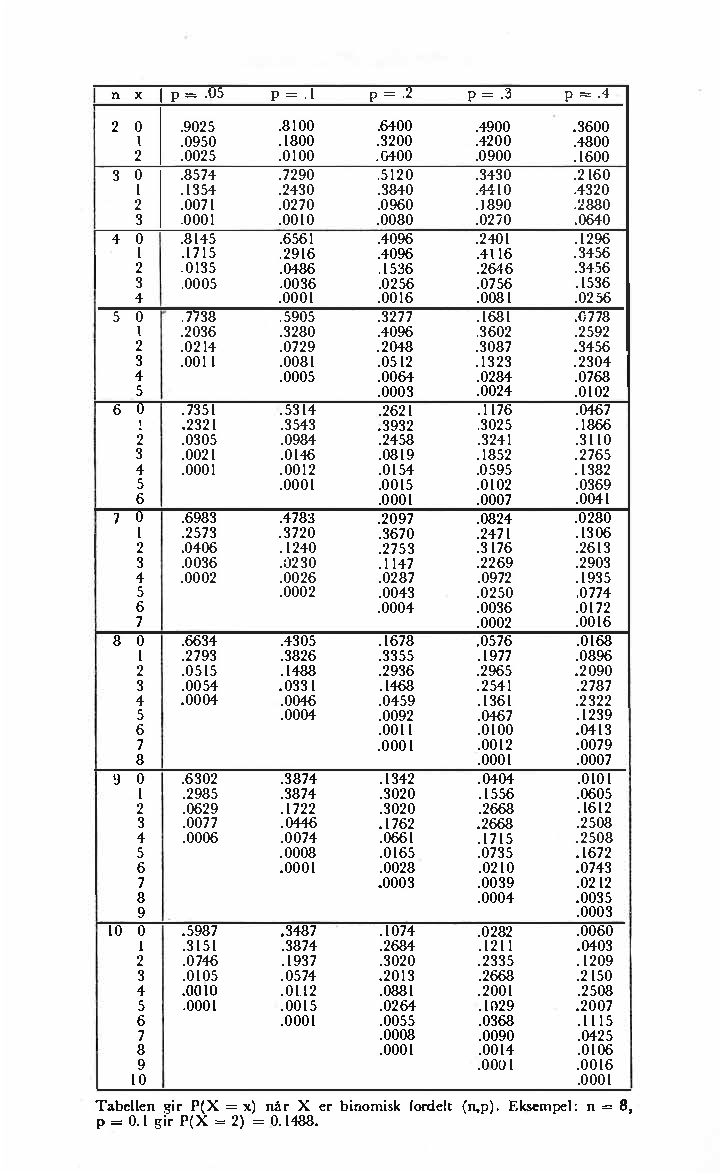
\includegraphics[scale=1.0]{figurer/Tabell_2a_Binomisk_fordeling.pdf}
 \caption{Binomisk fordeling}
 \label{tab:Binomisk_fordeling} % Tabell_2a
\end{table}


\begin{table}[H]
\centering
  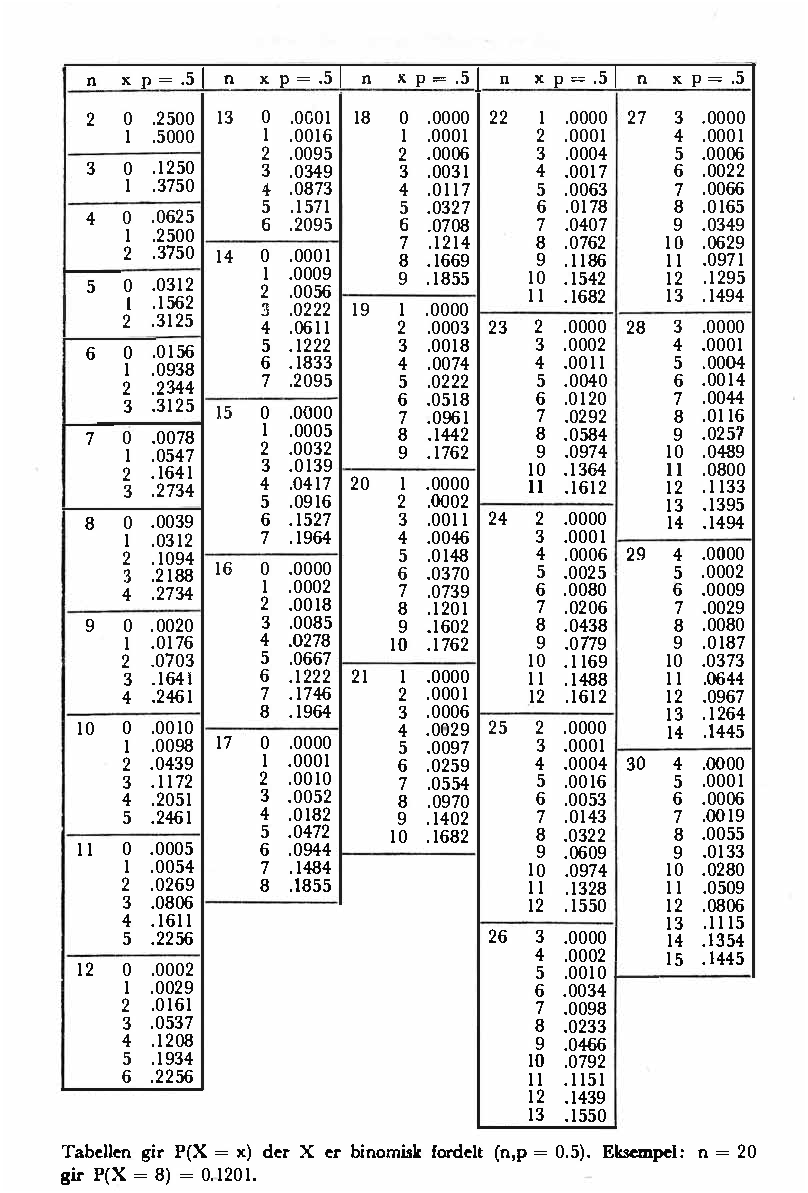
\includegraphics[scale=1.0]{figurer/Tabell_2b_Binomisk_fordeling.pdf}
 \caption{Binomisk fordeling $(p=0.5)$}
 \label{tab:Binomisk_fordeling_p05} % Tabell_2b
\end{table}

\begin{table}[H]
\centering
  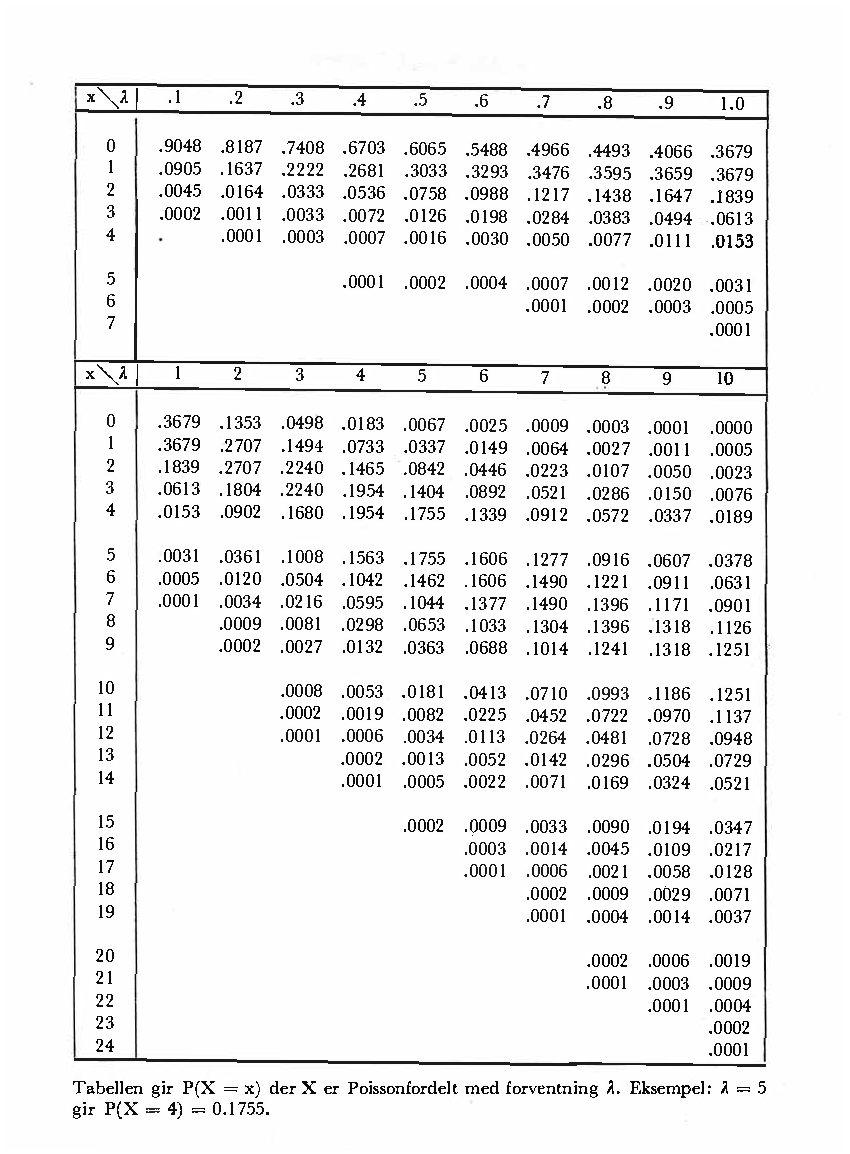
\includegraphics[scale=1.0]{figurer/Tabell_3_Poisson_fordeling.pdf}
 \caption{Poissonfordelingen}
 \label{tab:Poisson_fordeling} % Tabell_3
\end{table}

\begin{table}[H]
\centering
  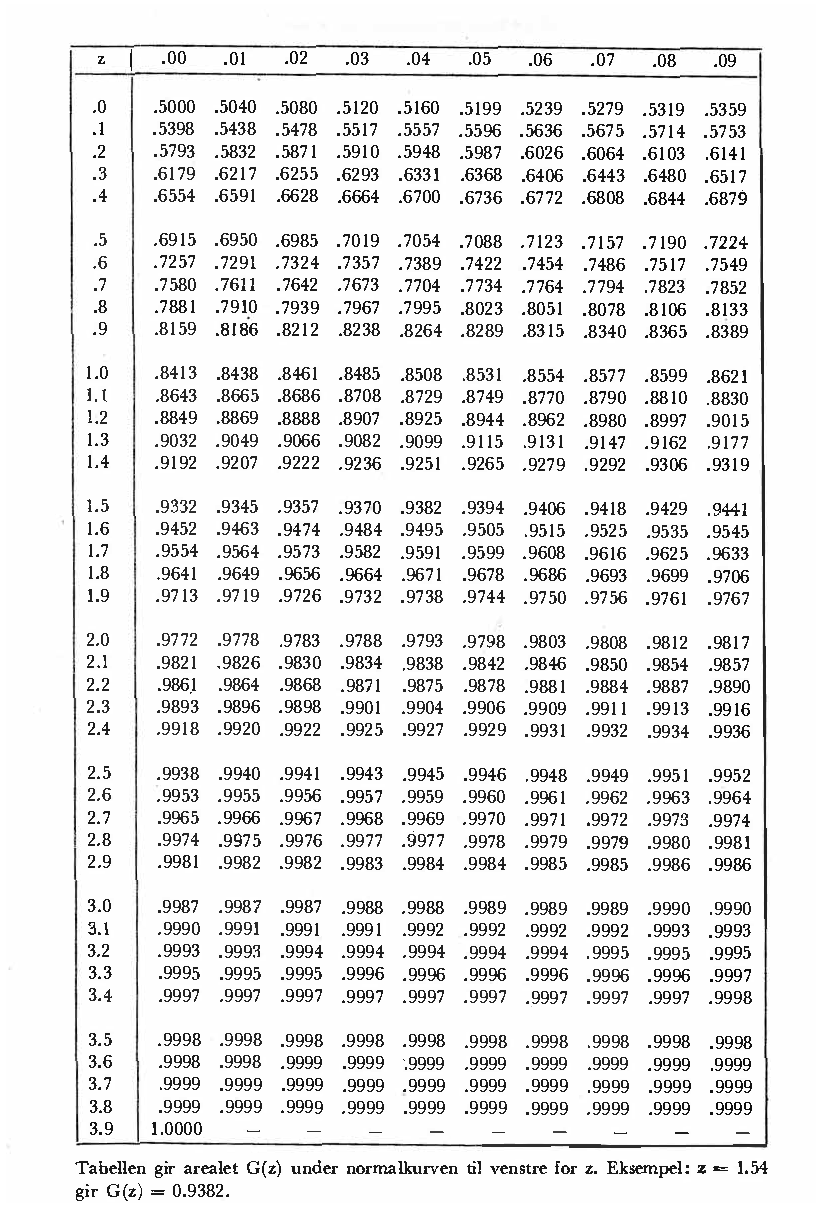
\includegraphics[scale=1.0]{figurer/Tabell_4a_Normal_Kurvenareal.pdf}
 \caption{Normalfordelingen (arealtabell)}
 \label{tab:Normal_Kurvenareal} % Tabell_4a
\end{table}

\begin{table}[H]
\centering
  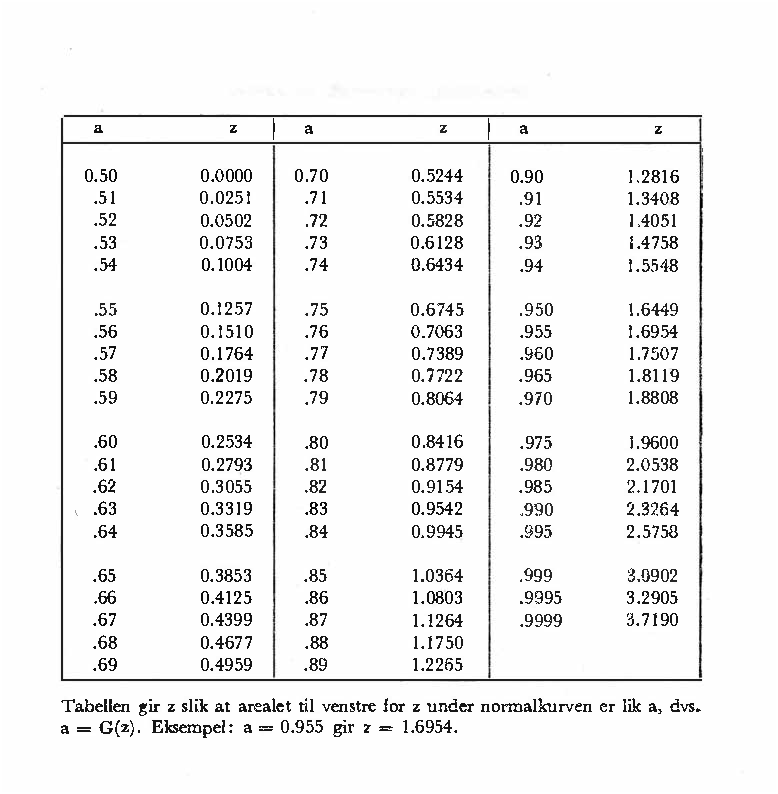
\includegraphics[scale=1.0]{figurer/Tabell_4b_Normal_Kurvefraktiler.pdf}
 \caption{Normalkurven (fraktiltabell)}
 \label{tab:Normal_Kurvefraktiler} % Tabell_4b
\end{table}

\begin{table}[H]
\centering
  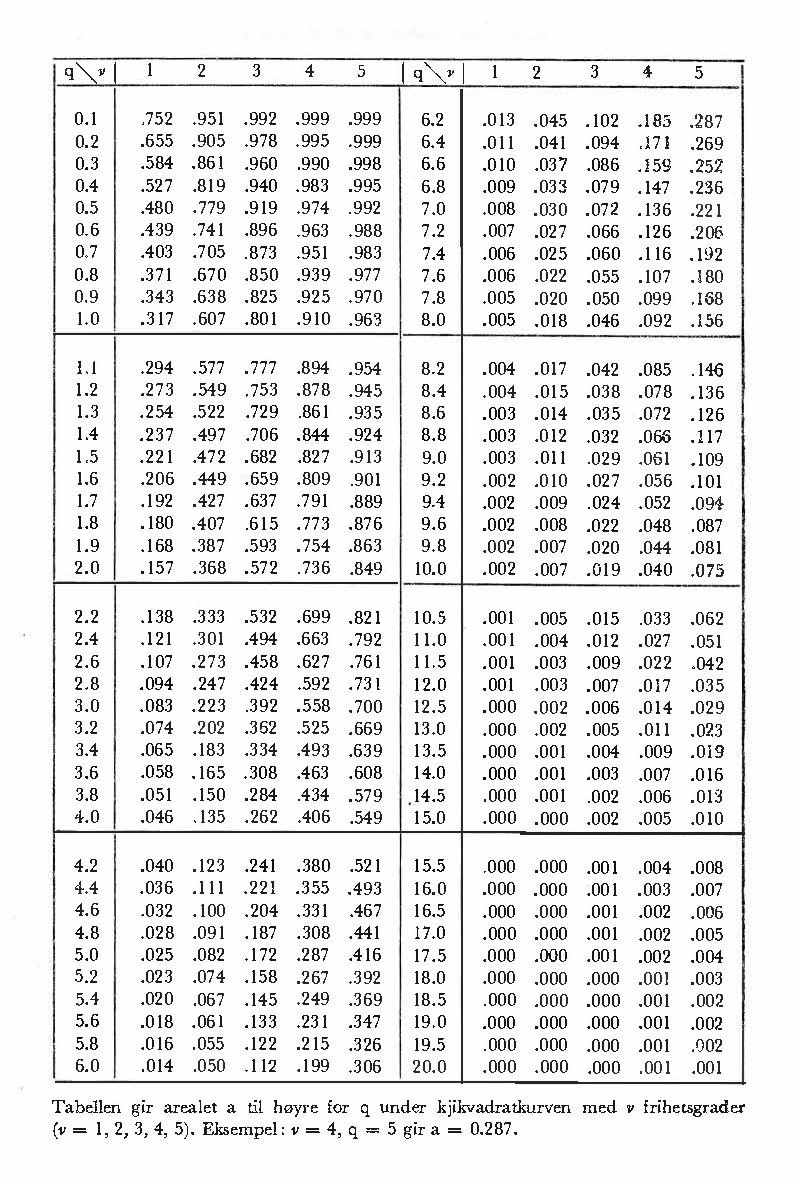
\includegraphics[scale=1.0]{figurer/Tabell_5a_Kjikvadrat_Areal.pdf}
 \caption{Kjikvadratkurver (arealtabell)}
 \label{tab:Kjikvadrat_Areal} % Tabell_5a
\end{table}

\begin{table}[H]
\centering
  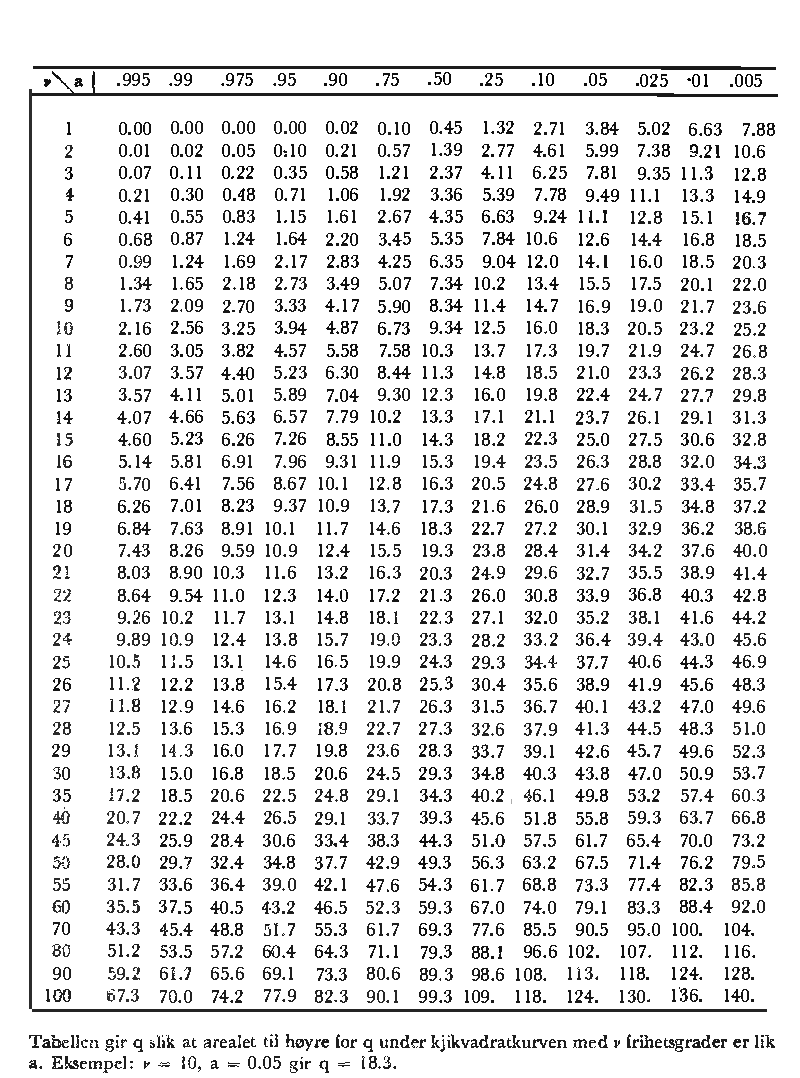
\includegraphics[scale=1.0]{figurer/Tabell_5b_Kjikvadrat_Fraktiler.pdf}
 \caption{Kjikvadratkurver (fraktiltabell)}
 \label{tab:Kjikvadrat_Fraktiler} % Tabell_5b
\end{table}

\begin{table}[H]
\centering
  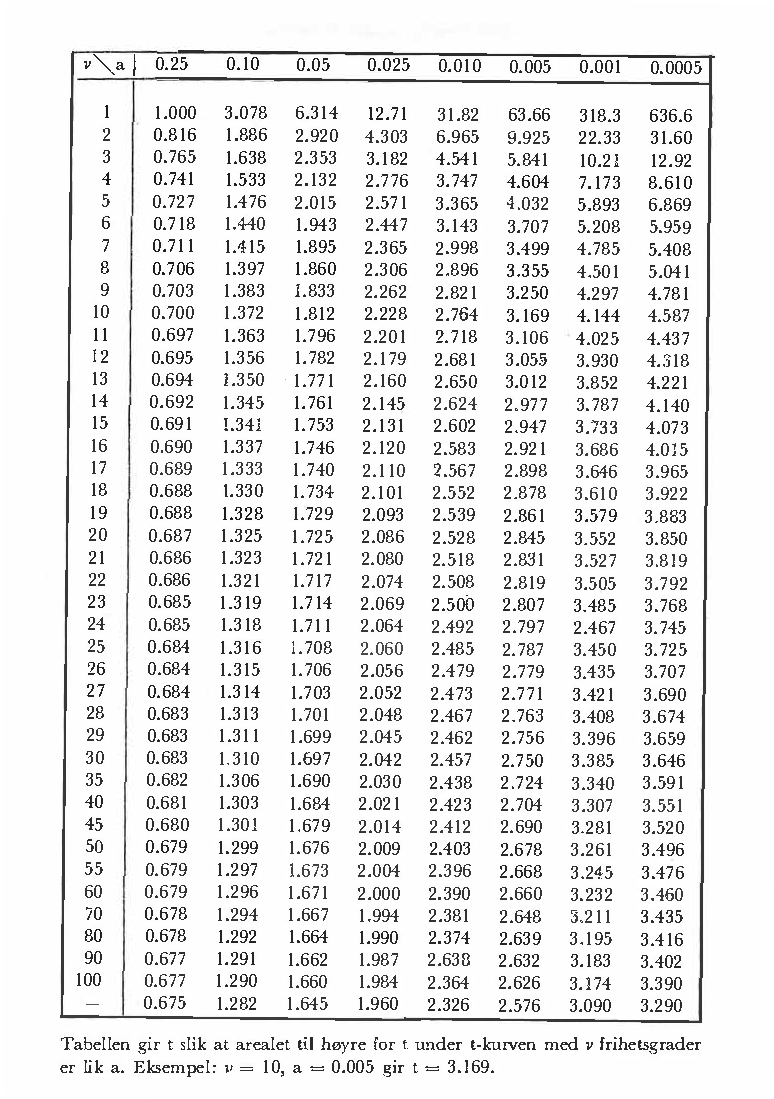
\includegraphics[scale=1.0]{figurer/Tabell_6_T_kurver_Fraktil.pdf}
 \caption{t-kurver (fraktiltabell)}
 \label{tab:T_kurver_Fraktil} % Tabell_6
\end{table}

\begin{table}[H]
\centering
  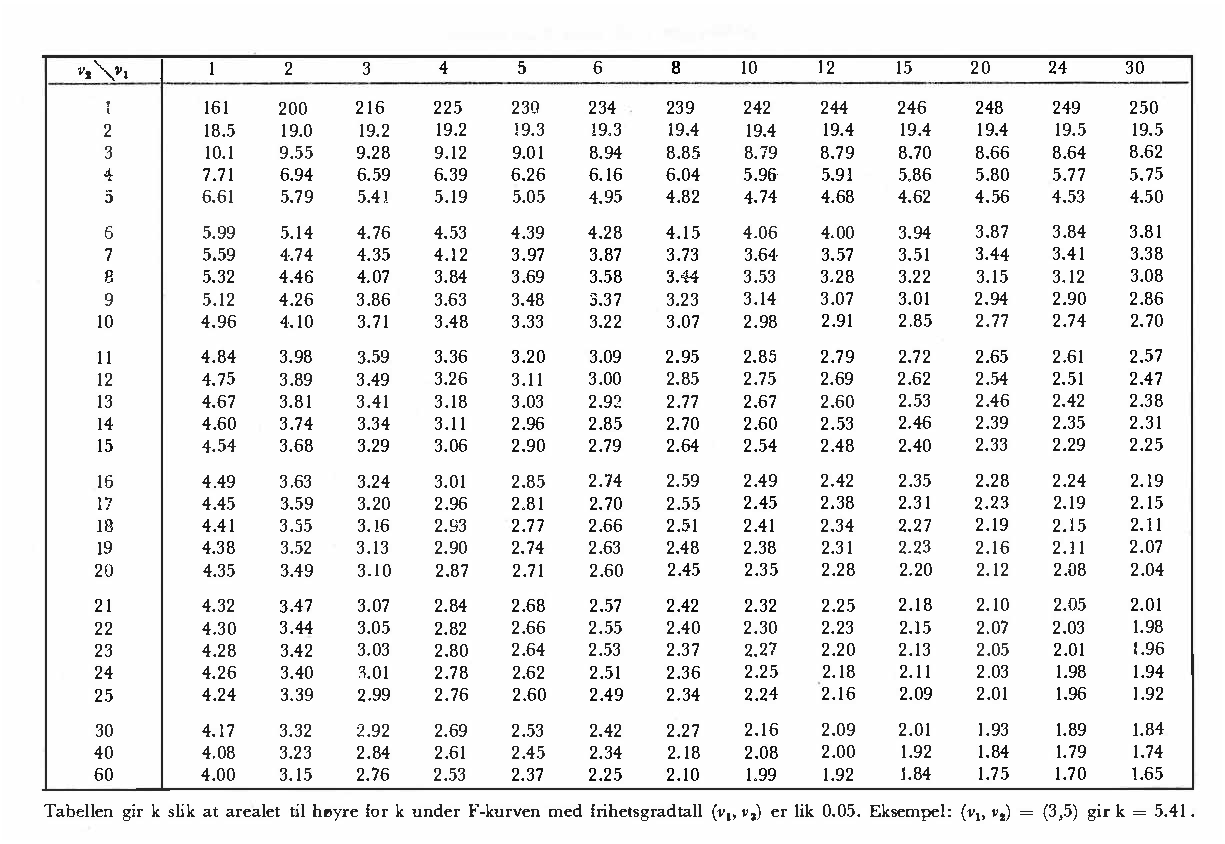
\includegraphics[scale=0.8]{figurer/Tabell_7a_F_kurver_Fraktiler_5_prosent.pdf}
 \caption{F-kurver (Øvre 5\%-fraktiler)}
 \label{tab:F_kurver_Fraktiler_5_prosent} % Tabell_7a
\end{table}

\begin{table}[H]
\centering
  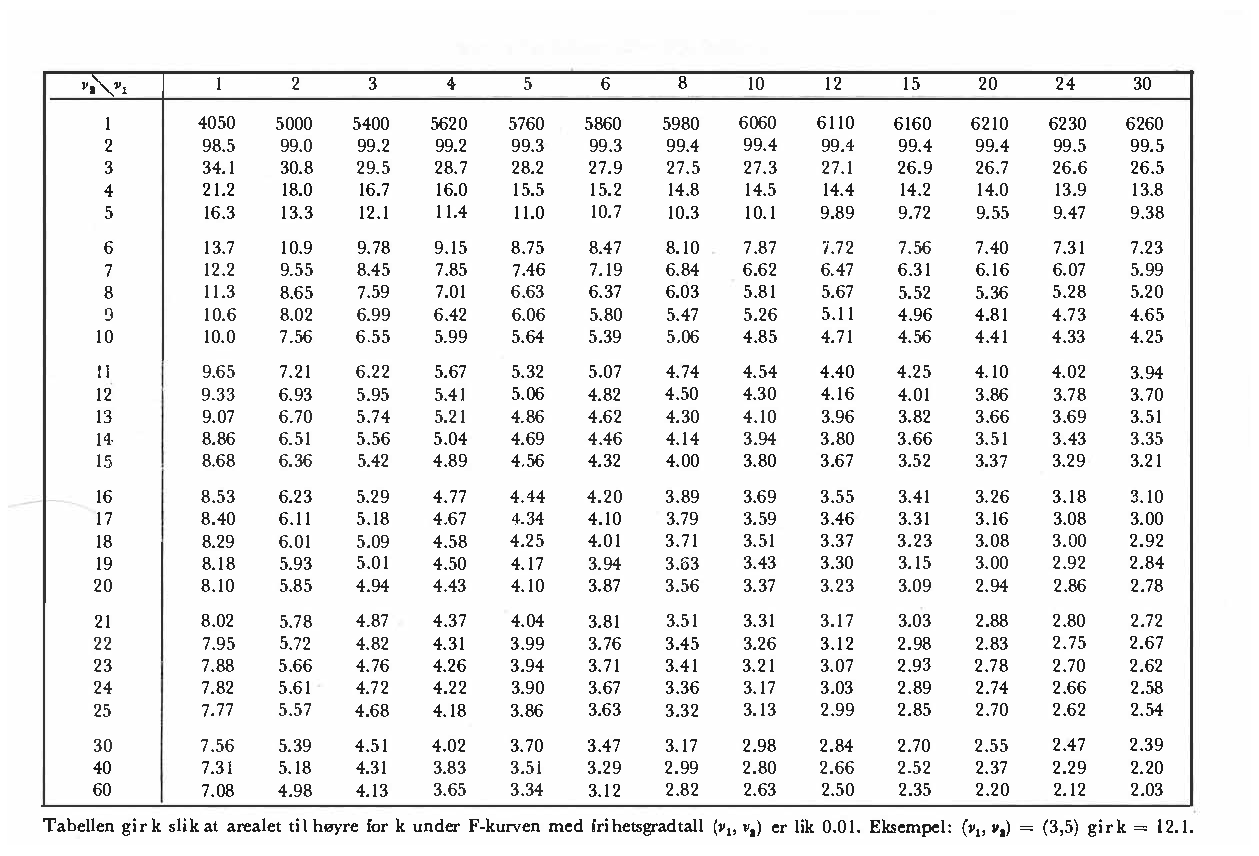
\includegraphics[scale=0.8]{figurer/Tabell_7b_F_kurver_Fraktiler_1_prosent.pdf}
 \caption{F-kurver (Øvre 1\%-fraktiler)}
 \label{tab:F_kurver_Fraktiler_1_prosent} % Tabell_7b
\end{table}

\begin{table}[H]
\centering
  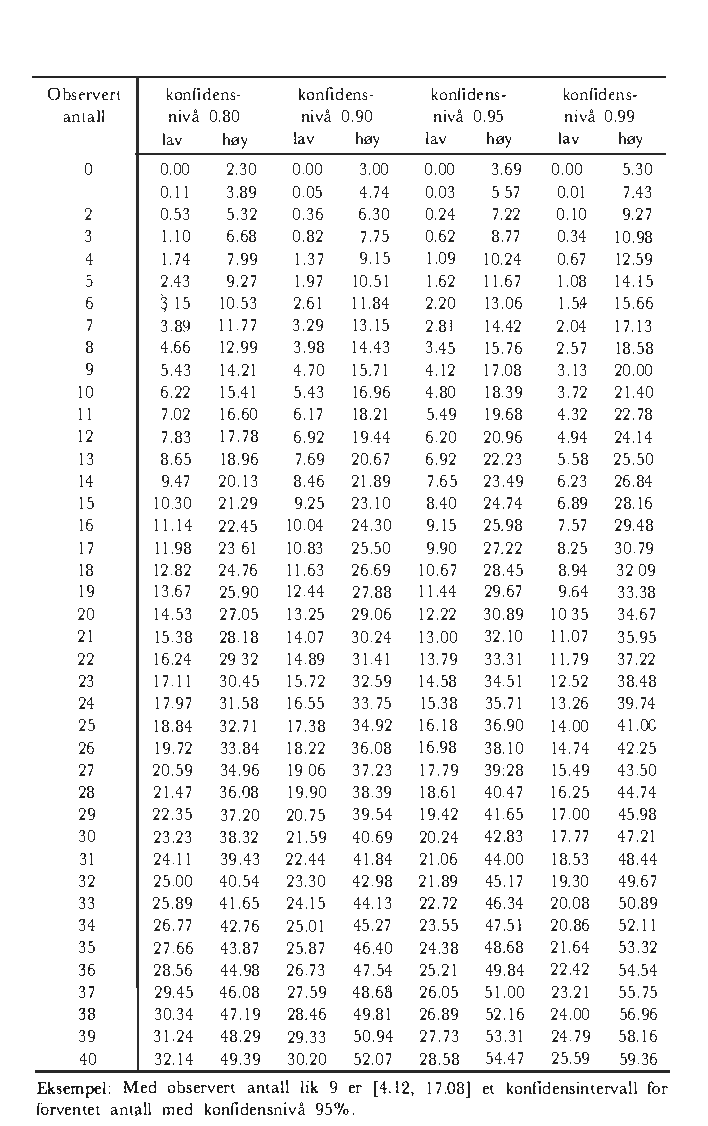
\includegraphics[scale=1.0]{figurer/Tabell_8_Konfidensgrenser_Poisson.pdf}
 \caption{Konfidensgrenser for Poissonforventning}
 \label{tab:Konfidensgrenser_Poisson} % Tabell_8
\end{table}

\begin{table}[H]
\centering
  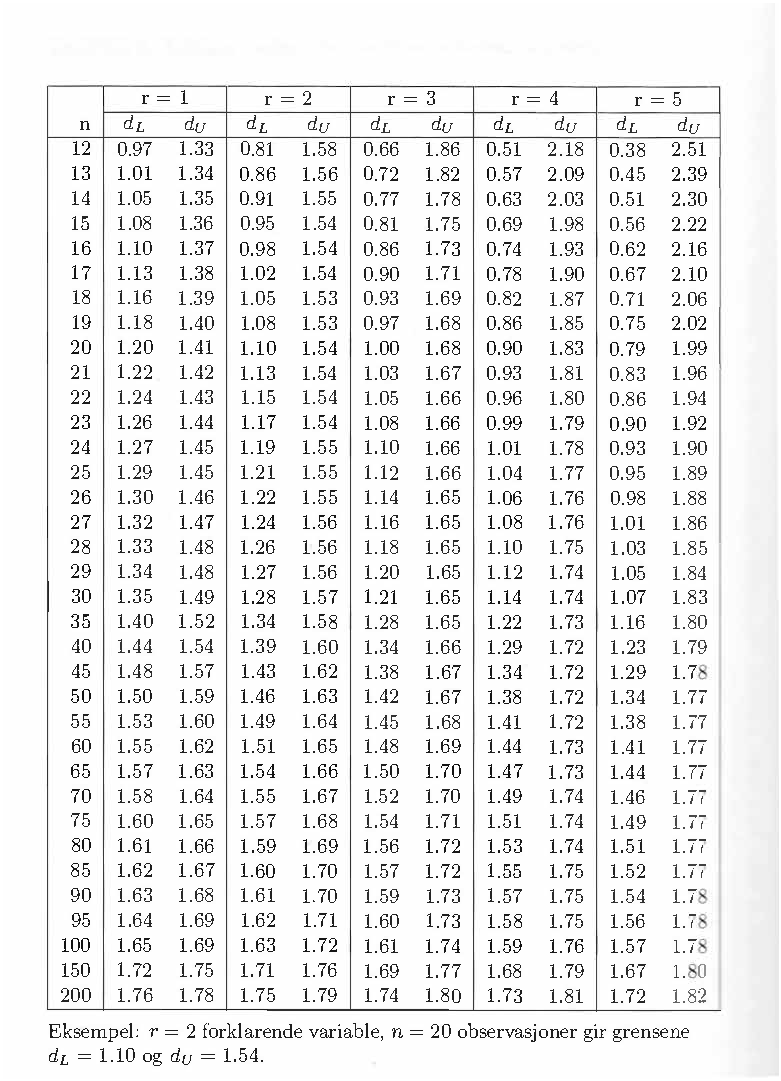
\includegraphics[scale=1.0]{figurer/Tabell_9_Durbin_Watson_test.pdf}
 \caption{Kritiske verdier Durbin-Watson testen (5\% nåvi)}
 \label{tab:Durbin_Watson_test} % Tabell_9
\end{table}

\noindent Av mer omfattende tabellverker anbefales:
\begin{itemize}
\item[] Odeh, Owen, Birnbaum \& Fisher:\\
        Pocket Book of Statistical Tables.\\
        Marcel Dekker, Basel 1977.
\item[] Owen:  Handbook of Statistical Tables.\\
        Addison Wesley, Reading Mass. 1962.
\item[] Pearson \& Hartley:  Biometrika Tables for Statisticians.\\
        Cambridge University Press, London 1962.
\end{itemize}
% \noindent samt spesialtabellene
% \begin{itemize}
% \item[] Lieberman \& Owen: \\ Tables of the Hypergeometric Probability
%        Distribution. \\
%        Stanford University Press, Stanford 1961.
% \item[] Tables of the Binomial Probability Distribution.\\
%        Harvard University Press, Cambridge Mass. 1955.
% \item[] Tables of the Individual and Cumulative Terms of Poisson
%        Distribution.\\
%        Van Nostrand, Princeton 1962.
% \item[] Rand Corporation: A Million Random Digits. \\ 
%        The Free Press, New York 1955.
% \end{itemize}
